\subsection{Arten von Softwarekomponenten}
\label{sec:2_Arten_Komponenten}

Verschiedene Arten von Komponenten können entsprechend ihren Aufgabenbereichen klassifiziert werden. Eine übersichtliche Art der Zuordnung von Aufgabenbereichen zu Komponenten kann auf der Basis der Trennung von Zuständigkeiten erfolgen, zum Beispiel auf der Basis einer Schichten-Architektur. Eine Schichten-Architektur dient der Trennung von Zuständigkeiten und einer losen Kopplung der Komponenten. Sie unterteilt ein Software-System in mehrere horizontale Schichten, wobei das Abstraktionsniveau der einzelnen Schichten von oben nach unten zunimmt. Eine jede Schicht bietet der unter ihr liegenden Schicht Schnittstellen an, über die diese auf sie zugreifen kann. Abbildung \ref{sfig:2_Schichtenarchitektur_Gut} auf Seite \pageref{fig:2_Schichtenarchitektur} veranschaulicht eine valide Form dieses Architekturparadigma. Abbildung \ref{sfig:2_Schichtenarchitektur_Schlecht} auf Seite \pageref{fig:2_Schichtenarchitektur} hingegen visualisiert eine nicht valide Schichtenarchitektur, denn Komponente 3 benutzt die Schnittstelle von Komponente 1. Somit verstößt dieses Beispiel gegen den Punkt, dass jede Schicht der unter ihr liegenden Schicht ihre Schnittstellen anbietet. \citereset \autocite[siehe][S. 17-25]{Andresen.2003}.

\begin{figure}[h]
  \centering
  \subfloat[Aufrufe in einer Schichtenarchitektur]{
    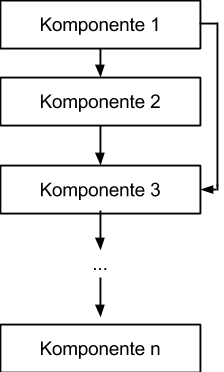
\includegraphics[height=5.0cm]{images/Schichtenarchitektur-Gut.png}
    \label{sfig:2_Schichtenarchitektur_Gut}
  }
  \qquad
  \subfloat[Verbotener Aufruf in einer Schichtenarchitektur]{
    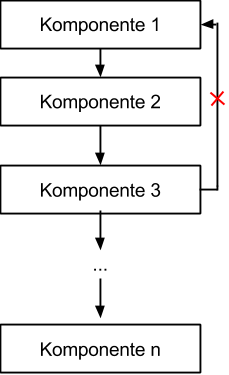
\includegraphics[height=5.0cm]{images/Schichtenarchitektur-Schlecht.png}
    \label{sfig:2_Schichtenarchitektur_Schlecht}
  }
  \caption[
    Beispiel einer Schichten-Architektur, Urldate: 04.2014 \newline
    \small\texttt{\url{http://www.oop-uml.de/drei-schichten-architektur.php}}
  ]{
    Beispiel einer Schichten-Architektur
  }
  \label{fig:2_Schichtenarchitektur}
\end{figure}

\begin{figure}[h]
\centering
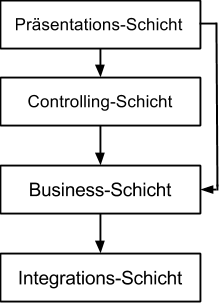
\includegraphics[height=5.0cm]{images/Schichtenarchitektur.png}
\caption[
Zuteilung der Komponenten
]{Zuteilung der Komponenten}
\label{fig:2_Schichtenarchitektur2}
\end{figure}

Auf Grundlage der in Abbildung \ref{fig:2_Schichtenarchitektur} auf Seite \pageref{fig:2_Schichtenarchitektur} veranschaulichten Architektur können Komponenten diversen Schichten zugeteilt werden, wie in Abbildung \ref{fig:2_Schichtenarchitektur2} auf Seite \pageref{fig:2_Schichtenarchitektur2} zu sehen ist:
\begin{enumerate}
\litem{Komponenten der Präsentations-Schicht} \hfill \\
Diese Komponenten stellen eine nach außen sichtbare Benutzerschnittstelle dar. Ein Beispiel dieser Schnittstelle ist eine GUI\footnote{Graphical User Interface}-Komponente (Button, Menü, Slider, und vieles mehr\ldots).
\litem{Komponenten der Controlling-Schicht} \hfill \\
Diese verarbeiten komplexe Ablauflogik und dienen als Vermittler zwischen Komponenten der Business- und Präsentations-Schicht. Ein Beispiel hierfür wäre ein Workflow-Controller. Er koordiniert die Interaktion mit einer oder mehreren Businesskomponenten. Diese Komponente kann zum Beispiel den Ablauf eines Geschäftsprozesses umsetzen.
\litem{Komponenten der Business-Schicht} \hfill \\
Sie bilden die Geschäftslogik im Sinne autonomer Businesskonzepte ab. Geschäftslogik in diesem Kontext bedeutet, dass die Komponente die Logik besitzt, die die eigentliche Problemstellung löst. Sie dient beispielsweise der Persistierung von Daten beziehungsweise bildet Entitäten auf Komponenten ab (Firma, Produkt, Kunden).
\litem{Komponenten der Integrations-Schicht} \hfill \\
Sie dient der Anbindung an Alt-Systeme, Fremd-Systeme und Datenspeicher. Dies könnten beispielsweise Connector-Komponenten oder Datenzugriffs-Komponenten sein. Connector-Komponenten dienen der Integration eines Fremd-Systems und Datenzugriffs-Komponenten liefert den Datenzugriff für Komponenten der oben genannten Schichten. Bei Datenzugriffs-Komponenten werden zum Beispiel die Besonderheiten einer Datenbank berücksichtigt.
\end{enumerate}

Komponente 1 in Abbildung \ref{fig:2_Schichtenarchitektur2} auf Seite \pageref{fig:2_Schichtenarchitektur2} würde hinsichtlich der genannten Einteilung die Präsentations-Schicht darstellen und somit der Nutzerin und dem Nutzer zur Interaktion und bereitstellen von Informationen dienen. Weiters würde Komponente 2 der genannten Abbildung die Controlling-Schicht repräsentieren. Die Präsentations-Schicht kann die vom Nutzer eingegebenen Daten der Controlling-Schicht weiterleiten. Diese würde sich mit Hilfe der zugrunde liegenden Business-Schicht (Komponente 3) um die Generierung von Antworten bezüglich der Nutzereingaben kümmern. Komponente 3, in diesem Beispiel die Business-Schicht, würde Aktivitäten zur Abwicklung eines Geschäftsprozesses ausführen oder Komponenten der Integrations-Schicht aktivieren. Die Komponenten können indirekt vom Nutzer über die Controlling-Schicht, von Komponenten der Integrations-Schicht oder aber von anderen Systemen aktiviert werden. Komponente 4 beziehungsweise die Integrations-Schicht ist für die Anbindung bestehender Systeme, Datenbanken und für die Nutzung spezifischer Middleware zuständig \citereset \autocite[siehe][S. 22-25]{Andresen.2003}.

Es ist zu erwähnen, dass es mehrere Kopplungen von Schichten-Architekturen gibt. Die in Abbildung \ref{sfig:2_Schichtenarchitektur_Gut} auf Seite \pageref{sfig:2_Schichtenarchitektur_Gut} verwendete Kopplung wird auch als \glqq lockere Schichten-Architektur\grqq\ bezeichnet. Zusätzlich zu dieser Kopplung gibt es noch eine \glqq reine\grqq , \glqq stärker gelockerte\grqq\ und \glqq vollständig gelockerte \grqq\ Schichten-Architektur. Diese Kopplungen werden nicht näher in dieser Arbeit erläutert.